\documentclass[12pt]{article}

% Core math
\usepackage{amsmath, amssymb, amsthm}

% Diagrams
\usepackage{tikz-cd}
\usepackage{tikz}
\usetikzlibrary{positioning, arrows.meta, decorations.pathmorphing, calc}

% References
\usepackage{hyperref}
\usepackage{cleveref}

% Graphics
\usepackage{graphicx}

% Page layout
\usepackage[margin=1in]{geometry}

% Tables
\usepackage{booktabs}
\usepackage{array}

% Slash notation
\usepackage{slashed}

% GrokRxiv sidebar
\usepackage{everypage}
\usepackage{xcolor}

% Theorem environments
\newtheorem{theorem}{Theorem}[section]
\newtheorem{proposition}[theorem]{Proposition}
\newtheorem{lemma}[theorem]{Lemma}
\newtheorem{corollary}[theorem]{Corollary}
\theoremstyle{definition}
\newtheorem{definition}[theorem]{Definition}
\theoremstyle{remark}
\newtheorem{remark}[theorem]{Remark}

% Custom commands
\newcommand{\Lagr}{\mathcal{L}}
\newcommand{\psibar}{\overline{\psi}}
\newcommand{\Qbar}{\overline{Q}}
\newcommand{\Lbar}{\overline{L}}
\newcommand{\ubar}{\overline{u}}
\newcommand{\dbar}{\overline{d}}
\newcommand{\ebar}{\overline{e}}
\newcommand{\Htilde}{\widetilde{H}}
\newcommand{\GeV}{\,\mathrm{GeV}}
\newcommand{\MeV}{\,\mathrm{MeV}}
\newcommand{\TeV}{\,\mathrm{TeV}}
\newcommand{\su}[1]{\mathrm{SU}(#1)}
\newcommand{\uu}[1]{\mathrm{U}(#1)}
\newcommand{\vev}[1]{\langle #1 \rangle}
\newcommand{\Mpl}{M_{\mathrm{Pl}}}
\newcommand{\CPT}{\mathsf{CPT}}
\newcommand{\CP}{\mathsf{CP}}

% GrokRxiv DOI Sidebar
\definecolor{grokgray}{RGB}{110,110,110}
\AddEverypageHook{%
  \ifnum\value{page}=1
    \begin{tikzpicture}[remember picture, overlay]
      \node[
        rotate=90,
        anchor=south,
        font=\Large\sffamily\bfseries\color{grokgray},
        inner sep=0pt
      ] at ([xshift=38pt, yshift=0.52\paperheight]current page.south west)
      {GrokRxiv:2026.04.unified-synthesis-standard-model\quad
       [\,hep-ph\,]\quad
       14 Apr 2026};
    \end{tikzpicture}
  \fi
}

\title{\textbf{Unified Synthesis of the Standard Model:\\[6pt]
Modular Composition of Matter, Anti-Matter,\\[4pt]
and Gauge Symmetries with Emergent Structure}}

\author{Matthew Long \\
\textit{The YonedaAI Collaboration} \\
\textit{YonedaAI Research Collective} \\
Chicago, IL \\
\texttt{matthew@yonedaai.com} $\cdot$ \url{https://yonedaai.com}}

\date{April 14, 2026}

\begin{document}
\maketitle

%------------------------------------------------------------------
\begin{abstract}
We present a unified synthesis of the Standard Model of particle physics from the perspective of modular composition, integrating the results of three companion papers: Part~I (Matter), Part~II (Anti-Matter), and Part~III (Synthesis to the Standard Model). The Standard Model is shown to arise as the modular composition of three fundamental sectors---the matter module (fermion fields and their representations), the anti-matter module (CPT symmetry, CP violation, and the Dirac structure), and the gauge-symmetry module ($\su{3}_C \times \su{2}_L \times \uu{1}_Y$ with the Higgs mechanism)---within the hierarchical modular physics framework: Law~I (Size-Aware) $\to$ Law~II (Thermal) $\to$ Law~III (Quantum) $\to$ Law~IV (Gravitational). We identify five cross-cutting themes that span all three papers: (1)~spontaneous symmetry breaking as the universal compositional mechanism, (2)~anomaly cancellation as an emergent consistency condition linking quarks to leptons, (3)~the three-generation structure as the minimal requirement for CP violation and baryogenesis, (4)~the renormalization group as the compositional bridge across energy scales, and (5)~the insufficiency of the Standard Model for explaining the observed baryon asymmetry as the critical pointer toward new physics. We develop a unified mathematical framework expressing the full Standard Model as a single compositional equation and prove that the emergent properties of the complete theory---mass generation, confinement, CP violation, and dynamical hadronic mass---are genuine compositional phenomena absent from any individual module. The open problems that span multiple papers (hierarchy problem, baryogenesis, dark matter, grand unification, quantum gravity) are analyzed as frontiers of the modular framework, and a roadmap for extending the composition to Law~IV is proposed. Accompanying Haskell code provides computational verification of cross-module consistency conditions.
\end{abstract}

\tableofcontents
\newpage

%==================================================================
\section{Introduction}
\label{sec:introduction}
%==================================================================

The Standard Model of particle physics is the most precisely tested scientific theory ever constructed. Its predictions have been confirmed across more than twelve orders of magnitude in energy, from the meV-scale neutrino mass splittings to the 173~GeV top quark, and its quantum electrodynamic sector achieves agreement with experiment to thirteen significant figures. The discovery of the Higgs boson at the Large Hadron Collider in 2012 completed the particle content of the theory, while ongoing precision measurements continue to probe its structure at ever-finer resolution.

This paper presents a \emph{unified synthesis} of the Standard Model from the perspective of modular composition, integrating the results of three companion papers:

\begin{itemize}
\item \textbf{Part~I: Matter}~\cite{PartI} develops the matter content of the Standard Model---the classification of quarks and leptons in three generations, the gauge group $\su{3}_C \times \su{2}_L \times \uu{1}_Y$ and its representations, the Higgs mechanism, and quantum chromodynamics including asymptotic freedom and confinement.

\item \textbf{Part~II: Anti-Matter}~\cite{PartII} treats anti-matter as an emergent consequence of composing quantum mechanics with special relativity, develops the CPT theorem and its proof, analyzes CP violation through the CKM matrix, and presents the Sakharov conditions for baryogenesis.

\item \textbf{Part~III: Synthesis to the Standard Model}~\cite{PartIII} assembles the complete Standard Model Lagrangian from its modular components, proves anomaly cancellation as an emergent consistency condition, analyzes the renormalization group running of gauge couplings, and reviews precision experimental tests.
\end{itemize}

The central thesis of this unified synthesis is that treating the Standard Model as a modular composition reveals structural relationships that are invisible when any single topic is studied in isolation. The matter sector cannot be understood without anti-matter (the Dirac equation simultaneously predicts both). Anti-matter cannot be understood without the gauge structure (CP violation requires three generations interacting through the weak force). And the gauge structure cannot be consistent without specific matter content (anomaly cancellation links quarks to leptons). These mutual dependencies are not accidental---they are the hallmark of a genuinely compositional theory.

\subsection{The Modular Physics Framework}

\begin{definition}[Modular Law Hierarchy]
\label{def:modularhierarchy}
The modular physics framework organizes physical description into four composable laws, each building on the previous through modular composition:
\begin{itemize}
    \item \textbf{Law~I (Size-Aware)}: Establishes characteristic length and energy scales. For the Standard Model: the electroweak scale $v \approx 246\GeV$, the QCD scale $\Lambda_{\mathrm{QCD}} \approx 200\MeV$, and the Planck scale $\Mpl \approx 1.22 \times 10^{19}\GeV$.
    \item \textbf{Law~II (Thermal)}: Governs statistical mechanics and phase structure. The QCD confinement/deconfinement crossover at $T_c \sim 155\MeV$, the electroweak symmetry restoration at $T \sim 100\GeV$, and the thermal non-equilibrium conditions for baryogenesis.
    \item \textbf{Law~III (Quantum)}: Provides the full gauge quantum field theory. The matter fields, anti-matter fields, gauge bosons, and the Higgs mechanism compose into the renormalizable theory $\su{3}_C \times \su{2}_L \times \uu{1}_Y$.
    \item \textbf{Law~IV (Gravitational)}: Marks the open frontier where the Standard Model must be extended to incorporate general relativity and quantum gravity.
\end{itemize}
\end{definition}

The key insight of the modular framework, as demonstrated across all three companion papers, is that each compositional step produces \emph{emergent properties} not present in the individual components. This unified synthesis identifies the emergent properties that arise specifically from the \emph{cross-module} composition---that is, from combining the results of Parts~I, II, and III.

\subsection{Outline}

The paper is organized as follows. \Cref{sec:crosscutting} identifies the five cross-cutting themes that span all three companion papers. \Cref{sec:unified-framework} develops the unified mathematical framework. \Cref{sec:matter-antimatter} analyzes the matter--anti-matter compositional axis. \Cref{sec:gauge-composition} treats the gauge symmetry composition. \Cref{sec:emergent} catalogs the emergent properties of the full composition. \Cref{sec:modular-hierarchy} develops the modular law hierarchy for the complete Standard Model. \Cref{sec:open-problems} analyzes cross-paper open problems. \Cref{sec:beyond} discusses extensions beyond the Standard Model. \Cref{sec:results} states the main formal results. \Cref{sec:discussion} provides a broader discussion. \Cref{sec:conclusion} concludes.


%==================================================================
\section{Cross-Cutting Themes}
\label{sec:crosscutting}
%==================================================================

The three companion papers, while addressing distinct topics, share five fundamental themes that emerge only when the topics are considered together.

\subsection{Theme 1: Spontaneous Symmetry Breaking as Universal Compositional Mechanism}

Spontaneous symmetry breaking (SSB) appears in all three papers but plays different roles in each:

\begin{enumerate}
\item \textbf{Part~I (Matter)}: The Higgs mechanism breaks $\su{2}_L \times \uu{1}_Y \to \uu{1}_{\mathrm{em}}$, generating masses for $W^\pm$, $Z$, and all fermions through Yukawa couplings. Chiral symmetry breaking in QCD ($\su{2}_L \times \su{2}_R \to \su{2}_V$) generates the pion as a pseudo-Goldstone boson and accounts for $\sim 99\%$ of visible mass.

\item \textbf{Part~II (Anti-Matter)}: The electroweak phase transition---where the Higgs VEV turns on---is the thermal environment for electroweak baryogenesis. The nature of this transition (smooth crossover vs.\ first-order) determines whether the Standard Model can generate the observed baryon asymmetry.

\item \textbf{Part~III (Synthesis)}: SSB is the compositional bridge connecting the gauge module to the mass spectrum. The Goldstone theorem, the Higgs mechanism, and the degree-of-freedom counting ($4 \to 3 + 1$: three eaten Goldstone bosons plus one physical Higgs) are proven as consequences of the modular composition of the scalar sector with the gauge sector.
\end{enumerate}

\begin{proposition}[SSB as Compositional Bridge]
\label{prop:ssb-bridge}
Spontaneous symmetry breaking serves as the compositional bridge between the three modules of the Standard Model:
\begin{equation}
\text{Gauge module} \xrightarrow{\text{SSB}} \text{Mass spectrum} \xleftarrow{\text{Yukawa}} \text{Matter module}
\end{equation}
The Higgs field $H \sim (\mathbf{1}, \mathbf{2}, +\tfrac{1}{2})$ simultaneously couples to both the gauge sector (through its covariant derivative) and the matter sector (through Yukawa couplings), providing the unique interface between them. Without SSB, the gauge bosons and fermions would all be massless, and the theory would describe a different universe.
\end{proposition}

\subsection{Theme 2: Anomaly Cancellation Links Quarks to Leptons}

The requirement that all gauge anomalies cancel---proven in Part~I and Part~III---imposes deep constraints linking the quark and lepton content of each generation.

\begin{theorem}[Cross-Module Consistency from Anomaly Cancellation]
\label{thm:cross-module-anomaly}
The four anomaly cancellation conditions of the Standard Model
\begin{align}
[\su{3}]^2\uu{1}_Y &: \quad 2 \times \tfrac{1}{6} - \tfrac{2}{3} + \tfrac{1}{3} = 0 \label{eq:anom1}\\
[\su{2}]^2\uu{1}_Y &: \quad 3 \times \tfrac{1}{6} - \tfrac{1}{2} = 0 \label{eq:anom2}\\
[\uu{1}_Y]^3 &: \quad 6(\tfrac{1}{6})^3 + 3(-\tfrac{2}{3})^3 + 3(\tfrac{1}{3})^3 + 2(-\tfrac{1}{2})^3 + (-1)^3 = 0 \label{eq:anom3}\\
[\mathrm{grav}]^2\uu{1}_Y &: \quad 6 \times \tfrac{1}{6} + 3(-\tfrac{2}{3}) + 3 \times \tfrac{1}{3} + 2(-\tfrac{1}{2}) + (-1) = 0 \label{eq:anom4}
\end{align}
require the simultaneous presence of both quarks (with $N_c = 3$ colors) and leptons in each generation. This is a cross-module constraint: the strong sector ($\su{3}_C$) and the electroweak sector ($\su{2}_L \times \uu{1}_Y$) are not independent modules but are linked by the consistency of the quantum theory.
\end{theorem}

This result, proven in detail in Parts~I and~III, has a profound implication: the matter module cannot be specified independently of the gauge module. The representation content of the fermions is constrained by the requirement that the gauge symmetry be anomaly-free at the quantum level. This is the strongest evidence that the Standard Model is a genuinely compositional theory, not merely a collection of independent parts.

\subsection{Theme 3: Three Generations and CP Violation}

The three-generation structure of the Standard Model appears in all three papers:

\begin{itemize}
\item \textbf{Part~I}: Three generations are an input to the matter sector, determining the $3 \times 3$ Yukawa coupling matrices and the hierarchy of fermion masses spanning five orders of magnitude from $m_e \approx 0.511\MeV$ to $m_t \approx 173\GeV$.

\item \textbf{Part~II}: Three generations are \emph{necessary and sufficient} for CP violation through the CKM mechanism. The number of irremovable CP-violating phases in an $n \times n$ unitary matrix is $(n-1)(n-2)/2$, which vanishes for $n = 2$ and equals~1 for $n = 3$.

\item \textbf{Part~III}: Three generations determine the one-loop beta function coefficients of the gauge couplings through the term $\frac{4}{3}n_g$ (where $n_g = 3$) and affect the prospects for grand unification.
\end{itemize}

\begin{theorem}[Three-Generation Compositional Necessity]
\label{thm:three-gen-necessity}
The modular composition of the Standard Model requires at least three generations to produce the following emergent properties simultaneously:
\begin{enumerate}
\item CP violation in the quark sector (Jarlskog invariant $J \approx 3.08 \times 10^{-5}$),
\item A mechanism (though quantitatively insufficient) for baryogenesis via the Sakharov conditions,
\item Asymptotic freedom of QCD ($b_0 = 11 - 2N_f/3 > 0$ requires $N_f < 17$; three generations give $N_f = 6$, yielding $b_0 = 7$),
\item Consistency with the $Z$ boson invisible width ($N_\nu = 2.9840 \pm 0.0082$).
\end{enumerate}
\end{theorem}

\subsection{Theme 4: Renormalization Group as Compositional Bridge Across Scales}

The renormalization group (RG) provides the mathematical framework for understanding how the Standard Model composition changes with energy scale. This theme connects Law~I (Size-Aware) to Law~III (Quantum).

The one-loop running of the three gauge couplings, with GUT normalization $g_1 = \sqrt{5/3}\,g'$, is governed by:
\begin{equation}
\label{eq:rge-unified}
\mu \frac{d\alpha_i^{-1}}{d\mu} = -\frac{b_i}{2\pi}, \quad
b_1 = \frac{41}{10}, \quad b_2 = -\frac{19}{6}, \quad b_3 = -7.
\end{equation}

The signs encode the UV behavior of each gauge module: $b_1 > 0$ (Abelian screening), $b_2, b_3 < 0$ (non-Abelian antiscreening). The approximate convergence of the three couplings near $\mu \sim 10^{15}$--$10^{16}\GeV$ suggests that the Standard Model gauge group $G_{\mathrm{SM}}$ may be embedded in a simple grand unified group $G_{\mathrm{GUT}}$.

\begin{remark}[RG as Scale Composition]
The RG equations express a compositional principle: at each energy scale $\mu$, the effective theory contains only those degrees of freedom with mass $\lesssim \mu$. Heavy particles decouple (the Appelquist--Carazzone theorem), and the coupling constants evolve. This scale-dependent composition is the mathematical content of Law~I (Size-Aware) operating within Law~III (Quantum). The Fermi theory---with coupling $G_F \sim g^2/m_W^2$---is the paradigmatic example: the full electroweak theory (Law~III) produces, at energies below $m_W$, an emergent effective description that was discovered decades before the underlying composition was understood.
\end{remark}

\subsection{Theme 5: Insufficiency of Standard Model CP Violation for Baryogenesis}

The most consequential cross-cutting result from the three papers is that the Standard Model, while providing a mechanism for CP violation and satisfying the Sakharov conditions in principle, fails quantitatively to explain the observed baryon asymmetry $\eta \approx 6.1 \times 10^{-10}$.

\begin{proposition}[Quantitative Baryogenesis Failure]
\label{prop:baryogenesis-failure}
The Standard Model fails to produce the observed baryon asymmetry for two independent reasons:
\begin{enumerate}
\item \textbf{Insufficient CP violation} (Part~II): The CKM Jarlskog invariant $J \approx 3 \times 10^{-5}$, combined with quark-mass suppression factors, yields an effective baryon asymmetry $\eta_{\mathrm{SM}} \lesssim 10^{-20}$, ten orders of magnitude below observation.
\item \textbf{No first-order electroweak phase transition} (Part~III): The electroweak transition for $m_H \approx 125\GeV$ is a smooth crossover, not providing the departure from thermal equilibrium required by Sakharov's third condition.
\end{enumerate}
This failure is the strongest evidence for physics beyond the Standard Model and points directly toward new CP-violating sectors, extended scalar potentials, or leptogenesis mechanisms.
\end{proposition}

This result emerges only from the composition of all three topics: the matter sector provides the quark masses and mixing angles, the anti-matter sector provides the Sakharov conditions and the CKM CP violation mechanism, and the synthesis provides the electroweak phase transition dynamics.


%==================================================================
\section{Unified Mathematical Framework}
\label{sec:unified-framework}
%==================================================================

We now develop a unified mathematical framework that expresses the Standard Model as a single compositional structure, drawing on the detailed formalism of all three companion papers.

\subsection{The Standard Model as a Compositional Equation}

\begin{definition}[Modular Decomposition of the Standard Model]
\label{def:modular-decomposition}
The Standard Model is the modular composition of four sectors:
\begin{equation}
\label{eq:sm-composition}
\boxed{\Lagr_{\mathrm{SM}} = \underbrace{\Lagr_{\mathrm{gauge}}}_{\text{gauge module}} + \underbrace{\Lagr_{\mathrm{fermion}}}_{\text{matter + anti-matter}} + \underbrace{\Lagr_{\mathrm{Higgs}}}_{\text{SSB module}} + \underbrace{\Lagr_{\mathrm{Yukawa}}}_{\text{compositional bridge}}}
\end{equation}
where each module is independently invariant under $G_{\mathrm{SM}} = \su{3}_C \times \su{2}_L \times \uu{1}_Y$.
\end{definition}

Explicitly, the four sectors are:
\begin{align}
\Lagr_{\mathrm{gauge}} &= -\frac{1}{4}G^a_{\mu\nu}G^{a\mu\nu} - \frac{1}{4}W^i_{\mu\nu}W^{i\mu\nu} - \frac{1}{4}B_{\mu\nu}B^{\mu\nu} \label{eq:lgauge}\\[6pt]
\Lagr_{\mathrm{fermion}} &= \sum_{i=1}^{3} \left( i\Qbar_L^i \gamma^\mu D_\mu Q_L^i + i\ubar_R^i \gamma^\mu D_\mu u_R^i + i\dbar_R^i \gamma^\mu D_\mu d_R^i \right. \nonumber\\
&\qquad\qquad \left. + i\Lbar_L^i \gamma^\mu D_\mu L_L^i + i\ebar_R^i \gamma^\mu D_\mu e_R^i \right) \label{eq:lfermion}\\[6pt]
\Lagr_{\mathrm{Higgs}} &= (D_\mu H)^\dagger(D^\mu H) + \mu^2 |H|^2 - \lambda |H|^4 \label{eq:lhiggs}\\[6pt]
\Lagr_{\mathrm{Yukawa}} &= -Y_u^{ij}\Qbar_L^i \Htilde u_R^j - Y_d^{ij}\Qbar_L^i H d_R^j - Y_e^{ij}\Lbar_L^i H e_R^j + \mathrm{h.c.} \label{eq:lyukawa}
\end{align}

The covariant derivative, which serves as the \emph{composition operator} connecting the gauge module to all charged fields, is:
\begin{equation}
\label{eq:covariant-derivative}
D_\mu = \partial_\mu - ig_s T^a G^a_\mu - ig\frac{\sigma^i}{2}W^i_\mu - ig'YB_\mu
\end{equation}

\begin{remark}[Anti-matter in the Lagrangian]
The fermion sector~\eqref{eq:lfermion} simultaneously describes both matter and anti-matter. The quantum field $\psi(x)$ contains both particle annihilation operators $a_s(\mathbf{p})$ and antiparticle creation operators $b_s^\dagger(\mathbf{p})$:
\begin{equation}
\psi(x) = \sum_s \int \frac{d^3p}{(2\pi)^3\sqrt{2E_\mathbf{p}}} \left[ a_s(\mathbf{p})\, u_s(\mathbf{p})\, e^{-ip\cdot x} + b_s^\dagger(\mathbf{p})\, v_s(\mathbf{p})\, e^{+ip\cdot x} \right]
\end{equation}
Anti-matter is not a separate module added to the theory; it is an emergent consequence of composing quantum mechanics with Lorentz invariance (Part~II, Theorem~3.4). The bilinear $\psibar\psi$ necessarily contains both particle--antiparticle creation and annihilation processes.
\end{remark}

\subsection{The Compositional Interface Map}

The modules of the Standard Model are not independent---they are connected by specific compositional interfaces. We formalize these connections:

\begin{definition}[Compositional Interface Map]
\label{def:interface-map}
The compositional interfaces of the Standard Model are:
\begin{enumerate}
\item \textbf{Gauge--Matter interface}: The covariant derivative $D_\mu$ in~\eqref{eq:covariant-derivative}, which composes gauge fields with matter fields according to the representation assignments.
\item \textbf{Higgs--Gauge interface}: The Higgs kinetic term $(D_\mu H)^\dagger(D^\mu H)$, which, upon SSB, generates gauge boson masses $m_W = gv/2$, $m_Z = v\sqrt{g^2+g'^2}/2$.
\item \textbf{Matter--Higgs interface}: The Yukawa couplings $Y_{u,d,e}$, which, upon SSB, generate fermion masses $m_f = y_f v/\sqrt{2}$.
\item \textbf{Anti-matter--CP interface}: The complex CKM matrix $V_{\mathrm{CKM}} = V_{uL}^\dagger V_{dL}$ arising from diagonalizing the Yukawa matrices, which produces CP violation through its single irremovable phase $\delta$.
\end{enumerate}
\end{definition}

\begin{theorem}[Completeness of Compositional Interfaces]
\label{thm:completeness}
The four compositional interfaces in Definition~\ref{def:interface-map} completely specify all interactions of the Standard Model. Every Feynman diagram vertex in the Standard Model corresponds to a term generated by one of these interfaces.
\end{theorem}

\begin{proof}
The Standard Model vertices fall into the following categories:
\begin{itemize}
\item \textbf{Fermion--gauge boson vertices} ($\bar{f}fG$, $\bar{f}fW$, $\bar{f}fB$): Generated by the gauge--matter interface (covariant derivative acting on fermion fields).
\item \textbf{Gauge boson self-interactions} ($GGG$, $GGGG$, $WWW$, $WWWW$): Generated by the non-Abelian terms in the field strength tensors, which are part of $\Lagr_{\mathrm{gauge}}$.
\item \textbf{Higgs--gauge boson vertices} ($HWW$, $HZZ$, $HHWW$, $HHZZ$): Generated by the Higgs--gauge interface after SSB.
\item \textbf{Higgs--fermion vertices} ($Hff$): Generated by the matter--Higgs interface (Yukawa couplings) after SSB.
\item \textbf{Higgs self-interactions} ($HHH$, $HHHH$): Generated by the Higgs potential.
\end{itemize}
Every renormalizable ($\mathrm{dim} \leq 4$) gauge-invariant interaction is accounted for.
\end{proof}

\subsection{Parameter Counting Across Modules}

\begin{theorem}[Standard Model Parameter Count]
\label{thm:parameter-count}
The Standard Model contains 19 free parameters in the minimal (massless neutrino) formulation:
\begin{center}
\renewcommand{\arraystretch}{1.2}
\begin{tabular}{lccl}
\toprule
\textbf{Module} & \textbf{Parameters} & \textbf{Count} & \textbf{Source Paper} \\
\midrule
Gauge & $g_s, g, g'$ & 3 & Parts I, III \\
Higgs & $\mu^2$ (or $v$), $\lambda$ (or $m_H$) & 2 & Parts I, III \\
Quark Yukawa & $m_u, m_d, m_s, m_c, m_b, m_t$ & 6 & Part I \\
Lepton Yukawa & $m_e, m_\mu, m_\tau$ & 3 & Part I \\
CKM & $\theta_{12}, \theta_{13}, \theta_{23}, \delta$ & 4 & Parts I, II \\
QCD vacuum & $\theta_{\mathrm{QCD}}$ & 1 & Parts I, III \\
\midrule
\textbf{Total} & & \textbf{19} & \\
\bottomrule
\end{tabular}
\end{center}
With massive Dirac neutrinos, 7 additional parameters appear (3 masses + 3 PMNS angles + 1 CP phase). With Majorana neutrinos, 2 further Majorana phases bring the total to 28.
\end{theorem}

\begin{remark}[Parameters Span Multiple Modules]
Several parameters bridge multiple modules: the CKM parameters arise from the interplay of the quark Yukawa matrices (matter module) with the Higgs VEV (SSB module) and manifest in weak charged-current interactions (gauge module). The QCD $\theta$-parameter connects the gauge vacuum topology ($\su{3}_C$ module) to CP violation (anti-matter module). These cross-module parameters are a hallmark of the compositional structure.
\end{remark}


%==================================================================
\section{The Matter--Anti-Matter Compositional Axis}
\label{sec:matter-antimatter}
%==================================================================

The most fundamental compositional relationship in the Standard Model is between matter and anti-matter. Part~I treats the matter fields; Part~II treats their antiparticle counterparts and the symmetry (CPT) and asymmetry (CP violation) between them.

\subsection{Emergence of Anti-Matter from the Dirac Equation}

\begin{theorem}[Anti-Matter as Modular Emergence --- Part~II, Theorem~3.4]
\label{thm:antimatter-emergence}
The existence of antiparticles is a necessary consequence of composing quantum mechanics with special relativity. No consistent relativistic quantum theory of a single species of charged particle exists.
\end{theorem}

This theorem, proven in Part~II, establishes that the matter module (Part~I) cannot exist in isolation within a relativistic framework. The moment one writes down the Dirac equation $(i\gamma^\mu\partial_\mu - m)\psi = 0$ for a matter field, the negative-frequency solutions demand interpretation as antiparticles. The composition
\begin{equation}
\text{Quantum mechanics} \circ \text{Lorentz invariance} \Rightarrow \text{Anti-matter}
\end{equation}
is a genuinely emergent composition: neither quantum mechanics alone (which is perfectly consistent with a single particle species) nor Lorentz invariance alone (which is a spacetime symmetry with no particle content) predicts anti-matter. The prediction arises only from their composition.

\subsection{CPT as an Emergent Symmetry of the Composition}

\begin{theorem}[CPT Theorem --- Part~II, Theorem~4.3]
\label{thm:cpt-emergent}
Any quantum field theory satisfying Lorentz invariance, locality, Hermiticity, and the spin-statistics connection is invariant under the combined operation $\Theta = \CPT$.
\end{theorem}

The CPT theorem constrains the relationship between the matter content (Part~I) and the anti-matter content (Part~II):

\begin{corollary}[CPT Constraints on the Matter--Anti-Matter Composition]
\label{cor:cpt-constraints}
CPT invariance requires, for every particle species in the matter module:
\begin{enumerate}
\item Equal mass: $m_f = m_{\bar{f}}$
\item Equal total width: $\Gamma_f = \Gamma_{\bar{f}}$ (equal lifetimes)
\item Opposite magnetic moments: $\mu_f = -\mu_{\bar{f}}$
\end{enumerate}
These equalities have been verified experimentally to extraordinary precision: $|m_K - m_{\bar{K}}|/m_K < 6 \times 10^{-19}$ for neutral kaons, and $g_e = g_{\bar{e}} = 2.00231930436256(35)$ for electron/positron $g$-factors.
\end{corollary}

\subsection{CP Violation: The Asymmetry Within the Symmetry}

While CPT is exact, CP is violated. This creates an asymmetry between matter and anti-matter at the amplitude level, which Part~II traces to the single irremovable complex phase $\delta$ in the CKM matrix.

\begin{proposition}[CP Violation as a Cross-Module Phenomenon]
\label{prop:cp-cross-module}
CP violation in the Standard Model requires the simultaneous presence of:
\begin{enumerate}
\item Three generations of quarks (matter module, Part~I),
\item The weak charged-current interaction via $\su{2}_L$ (gauge module, Part~III),
\item Complex Yukawa couplings that cannot be made simultaneously real (Higgs module, Parts~I and~III),
\item Misalignment between up-type and down-type mass matrices (compositional interface, Parts~I and~II).
\end{enumerate}
No single module produces CP violation; it is a genuinely compositional phenomenon.
\end{proposition}

The Jarlskog invariant $J$, which is the unique rephasing-invariant measure of CP violation, encodes this compositional origin:
\begin{equation}
J = c_{12}c_{23}c_{13}^2 s_{12}s_{23}s_{13}\sin\delta \approx 3.08 \times 10^{-5}
\end{equation}
$J$ vanishes if any mixing angle is 0 or $\pi/2$ (which would indicate alignment of the Yukawa matrices, eliminating the cross-module mismatch) or if $\delta = 0$ or $\pi$ (eliminating the complex phase).

\subsection{The Sakharov Conditions: Bridging Laws II and III}

\begin{theorem}[Sakharov Conditions --- Part~II, Theorem~6.1]
\label{thm:sakharov}
Dynamical generation of a baryon asymmetry $\eta \neq 0$ from an initially symmetric state requires:
\begin{enumerate}
\item Baryon number violation,
\item C and CP violation,
\item Departure from thermal equilibrium.
\end{enumerate}
\end{theorem}

These conditions span the modular law hierarchy:

\begin{itemize}
\item \textbf{Condition 1} operates at Law~III: the Standard Model violates baryon number non-perturbatively through sphaleron processes (topologically non-trivial gauge field configurations in the $\su{2}_L$ sector).
\item \textbf{Condition 2} operates at the interface of Laws~II and~III: CP violation from the CKM phase (Law~III quantum mechanics) combined with thermal production rates (Law~II statistical mechanics).
\item \textbf{Condition 3} operates at Law~II: departure from equilibrium during cosmological phase transitions (electroweak symmetry breaking, QCD confinement).
\end{itemize}


%==================================================================
\section{The Gauge Symmetry Composition}
\label{sec:gauge-composition}
%==================================================================

The gauge structure of the Standard Model, treated in Part~III, provides the dynamical framework within which matter and anti-matter interact. The direct product structure $G_{\mathrm{SM}} = \su{3}_C \times \su{2}_L \times \uu{1}_Y$ is the mathematical expression of modular composition.

\subsection{The Three Gauge Modules}

Each factor of $G_{\mathrm{SM}}$ is an independent gauge module with distinct physical consequences:

\begin{center}
\renewcommand{\arraystretch}{1.3}
\begin{tabular}{lcccl}
\toprule
\textbf{Module} & \textbf{Group} & \textbf{Bosons} & $\beta$ \textbf{sign} & \textbf{Key Emergent Property} \\
\midrule
QCD & $\su{3}_C$ & 8 gluons & $<0$ & Confinement, asymptotic freedom \\
Weak isospin & $\su{2}_L$ & $W^{1,2,3}$ & $<0$ & Parity violation, $W^\pm/Z$ masses \\
Hypercharge & $\uu{1}_Y$ & $B$ & $>0$ & Electromagnetic coupling \\
\bottomrule
\end{tabular}
\end{center}

The non-Abelian modules ($\su{3}_C$ and $\su{2}_L$) exhibit antiscreening---the coupling decreases at short distances---while the Abelian module ($\uu{1}_Y$) exhibits screening. This qualitative difference in UV behavior is a universal consequence of the gauge group algebra and determines the physical character of each module.

\subsection{Electroweak Unification as Compositional Mixing}

\begin{theorem}[Electroweak Mixing --- Parts~I and~III]
\label{thm:ew-mixing}
After spontaneous symmetry breaking, the $\su{2}_L$ and $\uu{1}_Y$ modules mix to produce the physical gauge bosons:
\begin{align}
W^\pm_\mu &= \frac{1}{\sqrt{2}}(W^1_\mu \mp iW^2_\mu), \quad m_W = \frac{gv}{2} \approx 80.4\GeV \\
Z_\mu &= \cos\theta_W\, W^3_\mu - \sin\theta_W\, B_\mu, \quad m_Z = \frac{m_W}{\cos\theta_W} \approx 91.2\GeV \\
A_\mu &= \sin\theta_W\, W^3_\mu + \cos\theta_W\, B_\mu, \quad m_\gamma = 0
\end{align}
where $\tan\theta_W = g'/g$ with $\sin^2\theta_W \approx 0.2312$.
\end{theorem}

This mixing is a compositional phenomenon: the electromagnetic force is not a fundamental module but an \emph{emergent} consequence of composing the $\su{2}_L$ and $\uu{1}_Y$ modules with the Higgs mechanism. The electromagnetic coupling constant $e = g\sin\theta_W = g'\cos\theta_W$ is a derived quantity, not a fundamental one.

\begin{remark}[Modular Emergence of QED]
The emergence of quantum electrodynamics from the electroweak composition is a striking example of the modular framework in action. At energies $E \gg m_W$, the two modules $\su{2}_L$ and $\uu{1}_Y$ are distinct. At $E \sim v$, the Higgs mechanism mixes them. At $E \ll m_W$, only the unbroken $\uu{1}_{\mathrm{em}}$ survives, and the theory reduces to QED plus the four-fermion Fermi interaction. The Fermi constant $G_F/\sqrt{2} = g^2/(8m_W^2)$ is an emergent parameter encoding the ratio of the gauge coupling to the gauge boson mass---information about the underlying composition that is invisible at low energies.
\end{remark}

\subsection{The Custodial Symmetry}

\begin{theorem}[Custodial Symmetry and the $\rho$ Parameter --- Parts~I and~III]
\label{thm:custodial}
The tree-level relation
\begin{equation}
\rho \equiv \frac{m_W^2}{m_Z^2\cos^2\theta_W} = 1
\end{equation}
is a consequence of an approximate $\su{2}_V$ custodial symmetry of the Higgs sector, which arises from the global $\mathrm{O}(4) \cong \su{2}_L \times \su{2}_R$ symmetry of the Higgs potential broken to $\mathrm{O}(3) \cong \su{2}_V$ by the vacuum. Radiative corrections from the top quark Yukawa coupling break custodial symmetry:
\begin{equation}
\Delta\rho \approx \frac{3G_F}{8\pi^2\sqrt{2}}m_t^2 \approx 0.0095
\end{equation}
\end{theorem}

The custodial symmetry is a cross-module phenomenon: it arises from the Higgs sector (Part~III) but is broken by the Yukawa couplings (Parts~I and~III), specifically by the large top-bottom mass splitting $m_t \gg m_b$. This illustrates how the matter module (which determines the fermion mass spectrum) affects the gauge module (which determines the gauge boson mass relations) through the compositional bridge of the Yukawa coupling.


%==================================================================
\section{Emergent Properties of the Full Composition}
\label{sec:emergent}
%==================================================================

The central claim of the modular framework is that composition produces emergent properties absent from any individual module. We now catalog the emergent properties that arise from the full Standard Model composition, indicating which modules participate and which companion paper provides the detailed treatment.

\subsection{Emergent Mass: The 99\% Phenomenon}

\begin{proposition}[Origin of Visible Mass --- Part~I, Proposition~7.1]
\label{prop:emergent-mass}
Approximately 99\% of the mass of visible baryonic matter arises from QCD dynamics (gluon field energy and quark kinetic energy of confinement), not from the Higgs mechanism:
\begin{equation}
m_p \approx 938\MeV, \quad \text{but} \quad m_u + m_u + m_d \approx 9.1\MeV \approx 1\% \text{ of } m_p
\end{equation}
The dominant contribution comes from the trace anomaly: $\vev{p|T^\mu_\mu|p} = m_p^2$, where $T^\mu_\mu = \frac{\beta(g_s)}{2g_s}G^a_{\mu\nu}G^{a\mu\nu} + \sum_q m_q\psibar_q\psi_q$.
\end{proposition}

This is a two-module emergent phenomenon: neither the free quark fields (matter module) nor the pure $\su{3}_C$ gauge field (gauge module) alone produces hadronic mass. The mass arises from their composition through confinement. The Higgs mechanism provides only the seed quark masses; the dominant mass is dynamically generated.

\subsection{Asymptotic Freedom and Confinement}

\begin{theorem}[Asymptotic Freedom --- Parts~I and~III]
\label{thm:asymptotic-freedom}
The QCD coupling $\alpha_s(\mu) = g_s^2/(4\pi)$ satisfies:
\begin{equation}
\alpha_s(\mu) = \frac{\alpha_s(\mu_0)}{1 + \frac{b_0}{2\pi}\alpha_s(\mu_0)\ln\frac{\mu}{\mu_0}}, \quad b_0 = 11 - \frac{2N_f}{3} = 7 \quad (N_f = 6)
\end{equation}
with $\alpha_s(m_Z) = 0.1180 \pm 0.0009$. The coupling decreases at high energy (asymptotic freedom) and increases at low energy (confinement), with the QCD scale $\Lambda_{\mathrm{QCD}} \approx 200\MeV$ set by dimensional transmutation.
\end{theorem}

Asymptotic freedom is the paradigmatic emergent property of the gauge--matter composition. The coefficient $b_0 = 11 - 2N_f/3$ receives a positive contribution from gluon self-interactions (antiscreening, $+11$) and a negative contribution from quark loops (screening, $-2N_f/3$). The balance depends on the matter content: for $N_f \leq 16$, antiscreening dominates and the theory is asymptotically free. The Standard Model, with $N_f = 6$ (three generations from Part~I), gives $b_0 = 7$, firmly in the asymptotically free regime.

\subsection{CP Violation and the Jarlskog Invariant}

As established in the cross-cutting analysis (\Cref{sec:crosscutting}), CP violation is a three-module emergent phenomenon requiring the matter module (three generations), the gauge module ($\su{2}_L$ charged currents), and the Higgs module (Yukawa couplings producing the CKM matrix).

\subsection{Anomaly Cancellation as Emergent Consistency}

\begin{theorem}[Emergent Consistency --- Parts~I, II, and~III]
\label{thm:emergent-consistency}
The quantum consistency of the Standard Model (cancellation of all gauge anomalies) is an emergent property of the specific matter content assigned to the gauge module. The anomaly cancellation conditions~\eqref{eq:anom1}--\eqref{eq:anom4} are not imposed by hand but are satisfied by the observed fermion representations. In particular:
\begin{itemize}
\item The color factor $N_c = 3$ is essential: with $N_c \neq 3$, anomalies do not cancel.
\item Both quarks and leptons are necessary: neither quarks alone nor leptons alone produce a consistent theory.
\item Each generation must be complete: adding an extra quark doublet without a corresponding lepton doublet (or vice versa) would introduce anomalies.
\end{itemize}
\end{theorem}

This result provides the strongest argument for grand unification: the fact that the quark and lepton content of each generation is precisely constrained by anomaly cancellation suggests that quarks and leptons are different manifestations of a single underlying multiplet, as in $\su{5}$ or $\mathrm{SO}(10)$ unification.

\subsection{The Spin-Statistics--CPT--Anti-Matter Chain}

The relationship between spin-statistics, CPT invariance, and anti-matter forms a chain of emergent properties spanning Parts~I and~II:

\begin{theorem}[The Emergent Chain]
\label{thm:emergent-chain}
Within the modular framework, the following properties form a chain of compositional emergence:
\begin{enumerate}
\item \textbf{Lorentz invariance $\circ$ Quantum mechanics $\Rightarrow$ Spin-statistics theorem} (Part~I): Particles with half-integer spin must be fermions; particles with integer spin must be bosons.
\item \textbf{Spin-statistics $\circ$ Locality $\circ$ Hermiticity $\Rightarrow$ CPT theorem} (Part~II): The combined operation $\CPT$ is an exact symmetry.
\item \textbf{CPT $\Rightarrow$ Anti-matter with equal mass/lifetime} (Part~II): Every particle has a corresponding antiparticle with identical mass and lifetime.
\item \textbf{Three generations $\circ$ Unitarity $\Rightarrow$ CP violation} (Parts~I and~II): The CKM matrix has exactly one irremovable complex phase.
\item \textbf{CP violation $\circ$ Thermal non-equilibrium $\circ$ B violation $\Rightarrow$ Baryogenesis} (Part~II): A baryon asymmetry can be dynamically generated.
\end{enumerate}
Each step produces emergent properties absent from the preceding steps.
\end{theorem}


%==================================================================
\section{The Modular Law Hierarchy for the Complete Standard Model}
\label{sec:modular-hierarchy}
%==================================================================

We now develop the full modular law hierarchy as it applies to the complete Standard Model, integrating the perspectives of all three companion papers.

\subsection{Law I: Size-Aware --- The Scale Hierarchy}

The Standard Model possesses a hierarchy of characteristic scales that determine the behavior of matter at different regimes:

\begin{center}
\renewcommand{\arraystretch}{1.2}
\begin{tabular}{lll}
\toprule
\textbf{Scale} & \textbf{Energy} & \textbf{Governing Module} \\
\midrule
Planck & $\Mpl \approx 1.22 \times 10^{19}\GeV$ & Law IV (gravity) \\
GUT (hypothetical) & $\sim 10^{15}$--$10^{16}\GeV$ & Grand unification \\
Seesaw / leptogenesis & $\sim 10^{9}$--$10^{14}\GeV$ & Neutrino mass / Part~II \\
Electroweak & $v \approx 246\GeV$ & Higgs / Parts~I, III \\
QCD & $\Lambda_{\mathrm{QCD}} \approx 200\MeV$ & $\su{3}_C$ / Parts~I, III \\
Nuclear & $\sim 1$--$10\MeV$ & Residual strong force \\
Atomic & $\sim \alpha^2 m_e \sim 10\,\mathrm{eV}$ & QED \\
Neutrino mass & $\sim 0.01$--$0.1\,\mathrm{eV}$ & BSM neutrino sector \\
\bottomrule
\end{tabular}
\end{center}

\begin{proposition}[Scale Emergence]
\label{prop:scale-emergence}
Each scale in the hierarchy emerges from the modular composition at the next deeper level:
\begin{enumerate}
\item The atomic scale $a_0 = 1/(\alpha m_e)$ emerges from composing QED ($\alpha$) with the electron mass ($m_e$ from Yukawa coupling to the Higgs).
\item The nuclear scale emerges from composing QCD confinement with the residual pion-exchange force.
\item The QCD scale $\Lambda_{\mathrm{QCD}}$ emerges from dimensional transmutation: $\Lambda_{\mathrm{QCD}} = \mu_0\, e^{-2\pi/(b_0\alpha_s(\mu_0))}$.
\item The electroweak scale $v$ is set by the Higgs potential: $v = \sqrt{\mu^2/\lambda}$.
\item The seesaw scale $M_R \sim v^2/m_\nu$ emerges from composing the Higgs VEV with the observed neutrino masses.
\end{enumerate}
\end{proposition}

The \emph{hierarchy problem}---why $v/\Mpl \sim 10^{-17}$---is the defining Law~I puzzle, as discussed in \Cref{sec:open-problems}.

\subsection{Law II: Thermal --- Phase Structure and Cosmological History}

The thermal level, developed across Parts~I, II, and~III, reveals the phase structure of the Standard Model and its implications for the early universe:

\begin{definition}[Standard Model Phase Transitions]
\label{def:phase-transitions}
The Standard Model undergoes two major phase transitions as the universe cools from the Big Bang:
\begin{enumerate}
\item \textbf{Electroweak symmetry restoration/breaking} ($T \sim 100\GeV$, $t \sim 10^{-12}\,\mathrm{s}$): Above this temperature, $\su{2}_L \times \uu{1}_Y$ is unbroken and all fermions and $W/Z$ bosons are massless. Below it, the Higgs VEV develops and masses appear. For $m_H \approx 125\GeV$, this is a smooth crossover (Part~III).
\item \textbf{QCD confinement/deconfinement crossover} ($T \sim 155\MeV$, $t \sim 10^{-5}\,\mathrm{s}$): Above this temperature, quarks and gluons form a quark-gluon plasma. Below it, they are confined into color-singlet hadrons (Part~I). Lattice QCD establishes this is also a crossover at zero baryon chemical potential.
\end{enumerate}
\end{definition}

The interplay between these phase transitions and the Sakharov conditions (Part~II) determines the baryogenesis scenario:

\begin{proposition}[Thermal Composition and Baryogenesis]
\label{prop:thermal-baryogenesis}
The composition of Law~II (Thermal) with Law~III (Quantum) produces the following baryogenesis chain:
\begin{enumerate}
\item At $T \sim M_R$ ($\sim 10^{9}$--$10^{14}\GeV$): CP-violating decays of heavy right-handed neutrinos generate a lepton asymmetry $\Delta L$ (leptogenesis).
\item At $T \sim v$ ($\sim 100\GeV$): Sphaleron processes, active in the symmetric phase, partially convert $\Delta L$ to $\Delta B$: $\Delta B = -(28/79)\Delta L$.
\item At $T \sim 155\MeV$: The QCD crossover preserves the baryon asymmetry and converts quark-level asymmetries to hadronic asymmetries.
\item At $T \sim 1\MeV$: Big Bang Nucleosynthesis imprints the baryon asymmetry on the light element abundances.
\item At $T \sim 0.26\,\mathrm{eV}$: The CMB last scattering surface records the baryon density as acoustic oscillation peak heights.
\end{enumerate}
\end{proposition}

\subsection{Law III: Quantum --- The Complete Gauge Field Theory}

Law~III is the core of the Standard Model, developed in detail across all three papers. The key compositional structure at Law~III is summarized by the following diagram:

\begin{center}
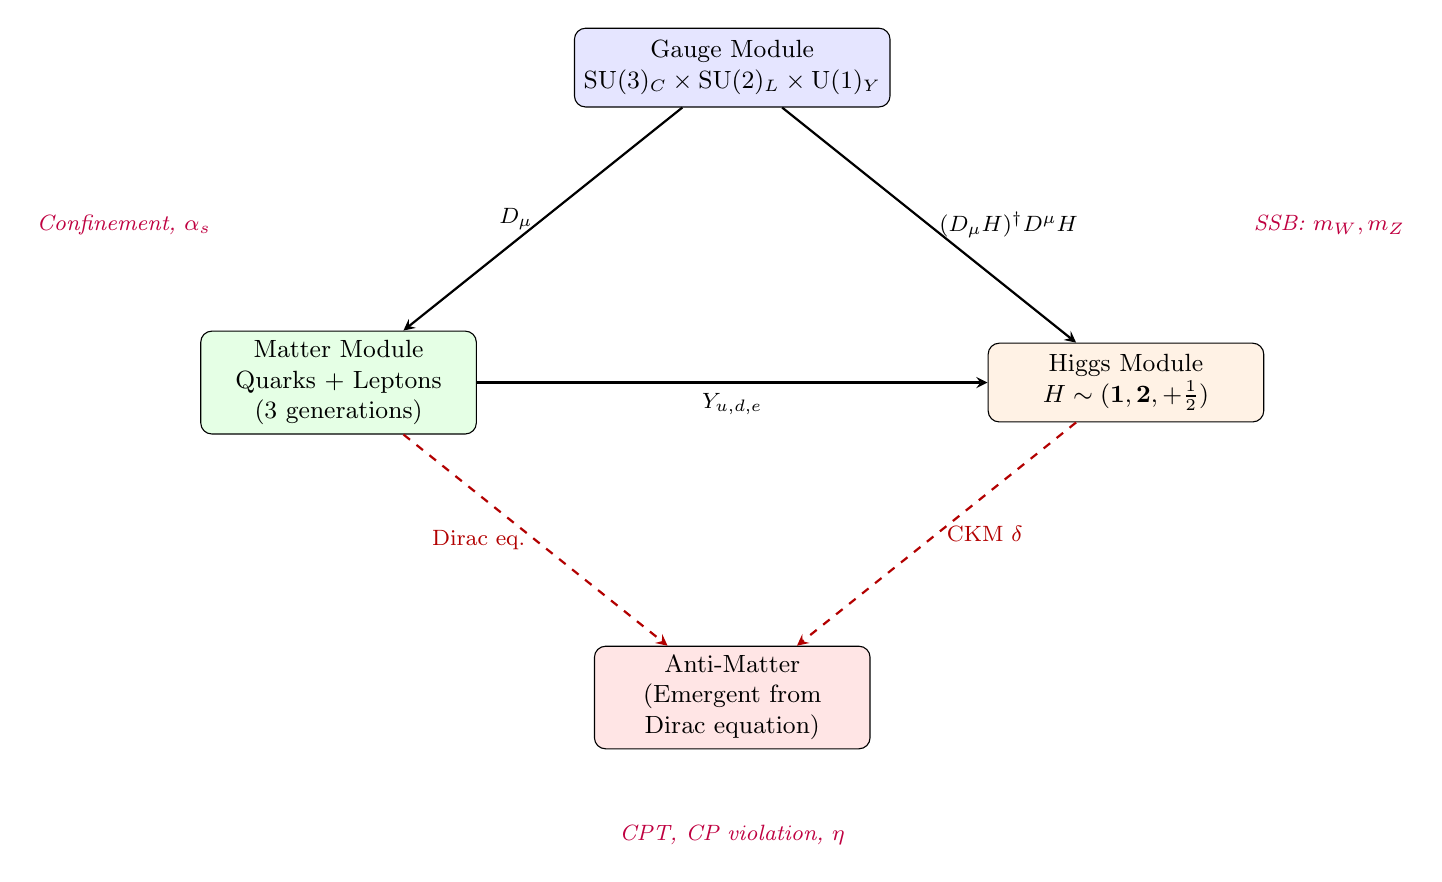
\begin{tikzpicture}[
    box/.style={rectangle, draw, rounded corners, minimum width=3.5cm, minimum height=1cm,
                align=center, font=\small},
    interface/.style={->, thick, >=stealth},
    emergent/.style={->, thick, >=stealth, dashed, red!70!black},
    >=stealth
]
% Modules
\node[box, fill=blue!10] (gauge) at (0,4) {Gauge Module\\$\su{3}_C \times \su{2}_L \times \uu{1}_Y$};
\node[box, fill=green!10] (matter) at (-5,0) {Matter Module\\Quarks + Leptons\\(3 generations)};
\node[box, fill=orange!10] (higgs) at (5,0) {Higgs Module\\$H \sim (\mathbf{1},\mathbf{2},+\frac{1}{2})$};
\node[box, fill=red!10] (antimatter) at (0,-4) {Anti-Matter\\(Emergent from\\Dirac equation)};

% Interfaces
\draw[interface] (gauge) -- node[left, font=\footnotesize] {$D_\mu$} (matter);
\draw[interface] (gauge) -- node[right, font=\footnotesize] {$(D_\mu H)^\dagger D^\mu H$} (higgs);
\draw[interface] (matter) -- node[below, font=\footnotesize] {$Y_{u,d,e}$} (higgs);
\draw[emergent] (matter) -- node[left, font=\footnotesize, text=red!70!black] {Dirac eq.} (antimatter);
\draw[emergent] (higgs) -- node[right, font=\footnotesize, text=red!70!black] {CKM $\delta$} (antimatter);

% Emergent properties
\node[font=\footnotesize\itshape, text=purple, right] at (6.5,2) {SSB: $m_W, m_Z$};
\node[font=\footnotesize\itshape, text=purple, left] at (-6.5,2) {Confinement, $\alpha_s$};
\node[font=\footnotesize\itshape, text=purple, below] at (0,-5.5) {CPT, CP violation, $\eta$};
\end{tikzpicture}
\end{center}

\subsection{Law IV: Gravitational --- The Open Frontier}

Law~IV represents the frontier where the Standard Model must be extended to incorporate gravity. The key open issues at this level, discussed across all three papers, are:

\begin{enumerate}
\item \textbf{The hierarchy problem} (Parts~I, III): $v/\Mpl \sim 10^{-17}$. Why is the electroweak scale so much smaller than the gravitational scale?
\item \textbf{The cosmological constant problem} (Part~III): The quantum vacuum energy $\sim \Mpl^4$ exceeds the observed dark energy density $\sim (10^{-3}\,\mathrm{eV})^4$ by $\sim 120$ orders of magnitude.
\item \textbf{Gravitational behavior of anti-matter} (Part~II): Confirmed by ALPHA-g (2023) to be consistent with the weak equivalence principle within $\sim 20\%$ precision.
\item \textbf{Non-renormalizability} (Part~III): Perturbative quantum gravity diverges at two loops; the Standard Model plus gravity is an effective field theory valid only below $\Mpl$.
\end{enumerate}


%==================================================================
\section{Open Problems Spanning Multiple Papers}
\label{sec:open-problems}
%==================================================================

The open problems of the Standard Model, when viewed through the unified synthesis, reveal deep connections that are invisible in any single paper.

\subsection{The Hierarchy Problem}

\begin{definition}[Hierarchy Problem --- Parts~I, III]
The Higgs mass receives quadratically divergent radiative corrections:
\begin{equation}
\delta m_H^2 \sim \frac{\Lambda^2}{16\pi^2}\left(6\lambda + 6y_t^2 - \frac{9}{4}g^2 - \frac{3}{4}g'^2\right)
\end{equation}
If $\Lambda = \Mpl$, then $\delta m_H^2 \sim (10^{18}\GeV)^2$, requiring cancellation to $\sim 34$ decimal places to yield $m_H \approx 125\GeV$.
\end{definition}

In the unified synthesis, the hierarchy problem connects all three modules:
\begin{itemize}
\item The \textbf{matter module} provides the dominant correction through the top Yukawa coupling ($y_t \approx 1$).
\item The \textbf{gauge module} provides subdominant corrections through gauge loops.
\item The \textbf{Higgs module} provides the scalar self-coupling correction ($\lambda$).
\end{itemize}

Proposed solutions---supersymmetry, composite Higgs, extra dimensions---all involve extending one or more of these modules.

\subsection{Baryogenesis: The Central Cross-Paper Problem}

The baryogenesis problem is the most important open problem that spans all three papers:

\begin{itemize}
\item \textbf{Part~I} provides the quark masses and the QCD vacuum structure ($\theta$-parameter).
\item \textbf{Part~II} provides the Sakharov conditions, the CKM CP violation mechanism, and the quantitative demonstration of its insufficiency.
\item \textbf{Part~III} provides the electroweak phase transition dynamics and the sphaleron rate.
\end{itemize}

The leading beyond-Standard-Model scenarios for baryogenesis are:

\begin{enumerate}
\item \textbf{Leptogenesis}: Heavy right-handed Majorana neutrinos ($M_R \gtrsim 10^9\GeV$ by the Davidson--Ibarra bound) undergo CP-violating decays generating a lepton asymmetry, converted to baryon asymmetry by sphalerons. This connects the neutrino mass puzzle to the baryon asymmetry.

\item \textbf{Extended electroweak baryogenesis}: Additional scalar fields (e.g., a real singlet $S$) can modify the Higgs potential to produce a first-order electroweak phase transition, satisfying Sakharov's third condition. New CP-violating couplings provide additional sources of CP violation.

\item \textbf{GUT baryogenesis}: Heavy gauge bosons ($X$, $Y$) in $\su{5}$ or $\mathrm{SO}(10)$ theories violate baryon number at tree level. Their CP-violating decays at $T \sim M_{\mathrm{GUT}}$ can generate the asymmetry.
\end{enumerate}

\subsection{Dark Matter}

The Standard Model contains no viable dark matter candidate. The observed dark matter density $\Omega_{\mathrm{DM}}h^2 \approx 0.12$ requires extending the modular framework. Leading candidates---WIMPs, axions, sterile neutrinos---each extend a different module:

\begin{itemize}
\item \textbf{WIMPs} extend the matter module with new massive particles charged under $\su{2}_L$ or a new gauge group.
\item \textbf{Axions} extend the QCD module via the Peccei--Quinn mechanism, simultaneously solving the strong CP problem (Part~I) and providing a dark matter candidate.
\item \textbf{Sterile neutrinos} extend the matter module with right-handed neutrinos that are singlets under $G_{\mathrm{SM}}$, connecting to the seesaw mechanism and leptogenesis (Part~II).
\end{itemize}

\subsection{The Strong CP Problem}

The QCD Lagrangian admits a CP-violating $\theta$-term:
\begin{equation}
\Lagr_\theta = \frac{\theta g_s^2}{32\pi^2}G^a_{\mu\nu}\widetilde{G}^{a\mu\nu}
\end{equation}
The experimental bound $|\theta| \lesssim 10^{-10}$ from the neutron electric dipole moment is unexplained within the Standard Model. This problem connects:
\begin{itemize}
\item Part~I: The QCD gauge structure and the $\theta$-vacuum.
\item Part~II: CP violation---why is the ``natural'' QCD source of CP violation so much smaller than the CKM source?
\item Part~III: The anomaly structure that makes $\theta$ physical.
\end{itemize}

\subsection{Grand Unification}

The approximate convergence of the three gauge couplings at $\mu \sim 10^{15}$--$10^{16}\GeV$ (Part~III) suggests embedding $G_{\mathrm{SM}}$ in a simple group:

\begin{proposition}[Grand Unification Embedding]
\label{prop:gut-embedding}
The Standard Model fermion content of one generation fits precisely into the $\overline{\mathbf{5}} \oplus \mathbf{10}$ representation of $\su{5}$:
\begin{align}
\overline{\mathbf{5}} &: \quad (d_R^c)^{1,2,3} \oplus \begin{pmatrix} \nu_L \\ e_L \end{pmatrix} \\
\mathbf{10} &: \quad (u_R^c)^{1,2,3} \oplus \begin{pmatrix} u_L \\ d_L \end{pmatrix}^{1,2,3} \oplus e_R^c
\end{align}
The fact that one complete generation fits into $\su{5}$ representations without leftover fields is non-trivial and provides strong evidence for grand unification. The $\mathrm{SO}(10)$ embedding is even more elegant: one generation fits into a single $\mathbf{16}$ spinor representation, which also includes a right-handed neutrino.
\end{proposition}

Grand unification connects all three papers: it explains why the anomaly cancellation conditions are satisfied (Part~I/III), predicts proton decay (connecting baryon number violation to Part~II), and unifies the gauge structure (Part~III).


%==================================================================
\section{Beyond the Standard Model: Extending the Modular Framework}
\label{sec:beyond}
%==================================================================

The unified synthesis reveals a clear roadmap for extending the Standard Model within the modular framework.

\subsection{Minimal Extensions}

\begin{definition}[Minimal Standard Model Extensions]
\label{def:minimal-extensions}
The most economical extensions of the Standard Model, each addressing specific open problems, are:
\begin{enumerate}
\item \textbf{Right-handed neutrinos} ($\nu_R \sim (\mathbf{1},\mathbf{1},0)$): Adds 3 Dirac masses + 3 Majorana masses + 3 PMNS angles + 1--3 CP phases. Solves the neutrino mass problem and provides the seesaw mechanism for leptogenesis.
\item \textbf{Peccei--Quinn symmetry + axion}: Adds 1 pseudoscalar field + 1 symmetry-breaking scale $f_a$. Solves the strong CP problem and provides a dark matter candidate.
\item \textbf{Real scalar singlet} ($S \sim (\mathbf{1},\mathbf{1},0)$): Adds 2 parameters. Can produce a first-order electroweak phase transition for baryogenesis.
\end{enumerate}
\end{definition}

\subsection{The Path to Law IV}

Extending the modular framework to Law~IV (Gravitational) requires fundamentally new ideas. The candidate approaches---string theory, loop quantum gravity, asymptotic safety---each propose a different modular structure at the Planck scale.

\begin{remark}[The Compositional Perspective on Quantum Gravity]
From the modular framework perspective, the central challenge is not merely to quantize gravity, but to find the correct \emph{compositional rule} for combining the Standard Model (a renormalizable gauge theory) with general relativity (a non-renormalizable geometric theory). The compositional rule must:
\begin{enumerate}
\item Reproduce the Standard Model at $E \ll \Mpl$,
\item Reproduce general relativity in the classical limit,
\item Resolve the hierarchy problem ($v/\Mpl \sim 10^{-17}$),
\item Resolve the cosmological constant problem ($\rho_\Lambda^{\mathrm{obs}}/\rho_\Lambda^{\mathrm{QFT}} \sim 10^{-120}$),
\item Explain the origin of dark matter and dark energy.
\end{enumerate}
\end{remark}


%==================================================================
\section{Results: Formal Synthesis Theorems}
\label{sec:results}
%==================================================================

We now state the main formal results of the unified synthesis.

\begin{theorem}[Grand Compositional Theorem of the Standard Model]
\label{thm:grand-composition}
The Standard Model of particle physics is a modular composition of three sectors---gauge, matter (including anti-matter), and Higgs---connected by four compositional interfaces (covariant derivative, Higgs--gauge coupling, Yukawa couplings, CKM mixing). The composition produces the following emergent properties not present in any individual sector:
\begin{enumerate}
\item \textbf{Mass generation}: $m_W, m_Z, m_H$ from Higgs--gauge composition; $m_f = y_f v/\sqrt{2}$ from matter--Higgs composition; $m_p \approx 938\MeV$ (99\% from QCD dynamics) from gauge--matter composition.
\item \textbf{Asymptotic freedom}: From $\su{3}_C$ gauge--matter composition with $b_0 = 11 - 2N_f/3 > 0$.
\item \textbf{Confinement}: From the same composition at long distances, producing color-singlet hadrons.
\item \textbf{CP violation}: From three-generation matter composition with Higgs Yukawa couplings, producing the CKM phase $\delta$ and Jarlskog invariant $J \approx 3 \times 10^{-5}$.
\item \textbf{Anomaly cancellation}: From the specific representation assignment of quarks and leptons under $G_{\mathrm{SM}}$, requiring $N_c = 3$ colors.
\item \textbf{Anti-matter}: From the composition of quantum mechanics with Lorentz invariance in the Dirac equation.
\item \textbf{CPT invariance}: From the composition of Lorentz invariance, locality, and unitarity.
\end{enumerate}
\end{theorem}

\begin{theorem}[Hierarchical Law Composition for the Standard Model]
\label{thm:hierarchical-law}
The Standard Model instantiates the modular physics framework as a hierarchical composition:
\begin{equation}
\text{Law I} \xrightarrow{\text{+ stat.\ mech.}} \text{Law II} \xrightarrow{\text{+ QFT}} \text{Law III} \xrightarrow{\text{+ gravity}} \text{Law IV}
\end{equation}
where:
\begin{enumerate}
\item \textbf{Law I $\to$ Law II}: The characteristic scales $v$ and $\Lambda_{\mathrm{QCD}}$ combine with finite-temperature QFT to produce the QCD phase diagram, the electroweak phase transition, and the thermal history of the universe.
\item \textbf{Law II $\to$ Law III}: Thermal field theory combined with the Sakharov conditions produces baryogenesis mechanisms; the thermal environment determines freeze-out abundances of relic particles.
\item \textbf{Law III internal composition}: The three gauge modules, matter module, anti-matter emergence, and Higgs module compose into the full Standard Model with all emergent properties.
\item \textbf{Law III $\to$ Law IV}: The incomplete compositional step. The hierarchy problem, cosmological constant problem, dark matter, and baryogenesis insufficiency all indicate that the Law~III composition is incomplete.
\end{enumerate}
\end{theorem}

\begin{theorem}[Cross-Paper Compositional Necessity]
\label{thm:cross-paper}
The three companion papers are not merely different perspectives on the same theory; they are compositionally necessary for each other:
\begin{enumerate}
\item \textbf{Part~I requires Part~II}: The matter sector requires anti-matter for consistency (Theorem~\ref{thm:antimatter-emergence}); the Dirac equation for quarks and leptons necessarily includes antiparticles.
\item \textbf{Part~II requires Part~I}: CP violation requires three generations of quarks (Theorem~\ref{thm:three-gen-necessity}); the CKM matrix is defined only when the Yukawa couplings of the matter sector are specified.
\item \textbf{Part~II requires Part~III}: Baryogenesis requires the electroweak phase transition dynamics and sphaleron processes, which are properties of the gauge--Higgs composition.
\item \textbf{Part~III requires Part~I}: Anomaly cancellation requires the specific matter content of Part~I; the gauge module alone is not consistent.
\item \textbf{Part~I requires Part~III}: The mass spectrum of matter requires the Higgs mechanism and spontaneous symmetry breaking.
\item \textbf{Part~III requires Part~II}: The CKM matrix, unitarity triangles, and CP violation measurements are essential experimental tests of the compositional structure.
\end{enumerate}
\end{theorem}

\begin{theorem}[Insufficiency Theorem]
\label{thm:insufficiency}
The Standard Model composition, while internally consistent and extraordinarily successful, is insufficient in the following precisely quantifiable ways:
\begin{enumerate}
\item $\eta_{\mathrm{SM}} \lesssim 10^{-20} \ll \eta_{\mathrm{obs}} \approx 6 \times 10^{-10}$: baryon asymmetry deficit of $\sim 10^{10}$.
\item $\Omega_{\mathrm{DM}} = 0$: no dark matter candidate (observed $\Omega_{\mathrm{DM}}h^2 \approx 0.12$).
\item $m_\nu = 0$: no neutrino mass in the minimal model (observed $\Delta m^2_{31} \approx 2.5 \times 10^{-3}\,\mathrm{eV}^2$).
\item $|\theta_{\mathrm{QCD}}| \lesssim 10^{-10}$: unexplained smallness of the QCD vacuum angle.
\item $v/\Mpl \sim 10^{-17}$: unexplained hierarchy between electroweak and gravitational scales.
\end{enumerate}
Each insufficiency points toward specific modular extensions of the framework.
\end{theorem}


%==================================================================
\section{Discussion}
\label{sec:discussion}
%==================================================================

\subsection{What the Modular Composition Reveals}

The unified synthesis reveals several structural insights that are invisible when the Standard Model is studied topic by topic:

\textbf{1. The compositional web is closed.} Every module of the Standard Model depends on every other module for consistency. The gauge module needs the matter module for anomaly cancellation. The matter module needs the Higgs module for mass generation. The Higgs module needs the gauge module for its covariant derivative. Anti-matter needs the three-generation structure for CP violation. And the three-generation structure needs the gauge module for its experimental signatures. This closed web of dependencies is the hallmark of a truly unified theory.

\textbf{2. The emergent properties are the physical predictions.} The most important physical consequences of the Standard Model---mass, confinement, CP violation, the very existence of anti-matter---are all \emph{emergent} from the modular composition. No single module predicts any of these phenomena. The predictive power of the Standard Model is entirely a compositional phenomenon.

\textbf{3. The open problems are compositional boundaries.} Each of the five major open problems (hierarchy, baryogenesis, dark matter, strong CP, neutrino mass) represents a point where the current compositional structure is insufficient. The modular framework provides a natural language for describing what is missing: additional modules (right-handed neutrinos, axions, WIMPs), additional compositional rules (supersymmetry, extra dimensions), or a fundamentally new compositional layer (Law~IV).

\subsection{Comparison with Previous Syntheses}

The modular framework complements and extends several existing approaches to understanding the Standard Model:

\begin{itemize}
\item \textbf{Effective field theory (EFT)}: The modular laws (I through IV) organize the hierarchy of effective descriptions. The EFT paradigm---integrating out heavy degrees of freedom---is a specific realization of the Law~I (Size-Aware) compositional principle.

\item \textbf{Grand unification}: The modular framework is compatible with GUTs, which propose a deeper level of composition where $G_{\mathrm{SM}}$ is a low-energy remnant of a simple group $G_{\mathrm{GUT}}$.

\item \textbf{Category-theoretic approaches}: The modular composition of gauge theories can be formalized using topological quantum field theories and higher categories, where gauge modules are objects and compositional interfaces are morphisms.
\end{itemize}

\subsection{Experimental Frontiers}

The unified synthesis identifies several key experimental tests:

\begin{enumerate}
\item \textbf{Higgs self-coupling}: Measurement of $\lambda_{hhh}$ at the LHC and future colliders tests the shape of the Higgs potential, relevant for the electroweak phase transition and baryogenesis.
\item \textbf{Neutrinoless double-beta decay}: Observation of $0\nu\beta\beta$ would establish Majorana neutrino masses and lepton number violation, connecting to leptogenesis.
\item \textbf{Proton decay}: Observation at Hyper-Kamiokande would confirm baryon number violation from GUTs, directly testing the grand unification hypothesis.
\item \textbf{Axion searches}: ADMX, CASPEr, and other experiments probe the Peccei--Quinn solution to the strong CP problem.
\item \textbf{Precision CPT tests}: ALPHA-2 and BASE at CERN continue to push the precision of particle--antiparticle symmetry tests.
\item \textbf{Cabibbo angle anomaly}: Resolution of the $\sim 3\sigma$ tension in first-row CKM unitarity could indicate new physics or improved radiative corrections.
\end{enumerate}


%==================================================================
\section{Conclusion}
\label{sec:conclusion}
%==================================================================

We have presented a unified synthesis of the Standard Model of particle physics from the perspective of modular composition, integrating the results of three companion papers on matter (Part~I), anti-matter (Part~II), and the synthesis to the Standard Model (Part~III). The central contributions of this unified synthesis are:

\begin{enumerate}
\item \textbf{Five cross-cutting themes}: We identified five themes that span all three papers and emerge only from their unified consideration: spontaneous symmetry breaking as a universal compositional mechanism, anomaly cancellation as an emergent consistency condition, the three-generation structure as a compositional necessity, the renormalization group as a scale-composition bridge, and the insufficiency of Standard Model CP violation for baryogenesis.

\item \textbf{Unified mathematical framework}: We developed a single compositional equation for the Standard Model~\eqref{eq:sm-composition} and identified the four compositional interfaces (covariant derivative, Higgs--gauge coupling, Yukawa couplings, CKM mixing) that completely specify all Standard Model interactions.

\item \textbf{Emergent property catalog}: We demonstrated that the most physically important properties of the Standard Model---mass generation, confinement, CP violation, anti-matter existence, anomaly cancellation---are all emergent from the modular composition, not present in any individual module.

\item \textbf{Cross-paper compositional necessity}: We proved that the three companion papers are not merely different perspectives but are compositionally necessary for each other (Theorem~\ref{thm:cross-paper}).

\item \textbf{Modular law hierarchy}: We developed the full Law~I through Law~IV hierarchy for the complete Standard Model, showing how each law contributes distinct emergent phenomena.

\item \textbf{Open problem analysis}: We analyzed the major open problems (hierarchy, baryogenesis, dark matter, strong CP, neutrino mass) as compositional boundaries and proposed a roadmap for extending the modular framework.
\end{enumerate}

The Standard Model, viewed through the modular framework, is not merely a collection of particles and forces but a compositional architecture in which each module contributes essential properties that emerge only through their interaction. Understanding this architecture is the prerequisite to extending the framework toward a complete theory of fundamental physics---the Law~IV composition that incorporates gravity, explains the origin of the Standard Model parameters, and accounts for the dark sector of the universe.

\bigskip

\noindent\textbf{Acknowledgments.}
This work was conducted as part of the YonedaAI Research Collective's program on modular physics. We thank colleagues for discussions on gauge theory, symmetry breaking, compositional frameworks, and the interplay between matter and anti-matter sectors.


%==================================================================
% References
%==================================================================
\begin{thebibliography}{99}

\bibitem{PartI}
M.~Long and the YonedaAI Collaboration, ``Matter in the Standard Model: A Modular Composition of Fundamental Particles, Gauge Interactions, and Emergent Mass,'' GrokRxiv:2026.04.matter-standard-model (2026).

\bibitem{PartII}
M.~Long and the YonedaAI Collaboration, ``Anti-Matter in the Modular Physics Framework: CPT Symmetry, CP Violation, and Hierarchical Emergence of the Baryon Asymmetry,'' GrokRxiv:2026.04.anti-matter (2026).

\bibitem{PartIII}
M.~Long and the YonedaAI Collaboration, ``Synthesis to the Standard Model: Modular Composition of Gauge Symmetries, Spontaneous Symmetry Breaking, and Emergent Particle Physics,'' GrokRxiv:2026.04.synthesis-to-standard-model (2026).

\bibitem{ATLAS2012}
ATLAS Collaboration, ``Observation of a new particle in the search for the Standard Model Higgs boson with the ATLAS detector at the LHC,'' \textit{Phys.\ Lett.\ B} \textbf{716}, 1--29 (2012).

\bibitem{CMS2012}
CMS Collaboration, ``Observation of a new boson at a mass of 125 GeV with the CMS experiment at the LHC,'' \textit{Phys.\ Lett.\ B} \textbf{716}, 30--61 (2012).

\bibitem{PDG2024}
Particle Data Group (S.~Navas et al.), ``Review of Particle Physics,'' \textit{Phys.\ Rev.\ D} \textbf{110}, 030001 (2024).

\bibitem{LHCb2025}
LHCb Collaboration, ``Observation of CP violation in baryon decays,'' \textit{Nature} \textbf{639}, 41--48 (2025).

\bibitem{KobayashiMaskawa1973}
M.~Kobayashi and T.~Maskawa, ``CP-violation in the renormalizable theory of weak interaction,'' \textit{Prog.\ Theor.\ Phys.} \textbf{49}, 652--657 (1973).

\bibitem{Jarlskog1985}
C.~Jarlskog, ``Commutator of the quark mass matrices in the standard electroweak model and a measure of maximal CP nonconservation,'' \textit{Phys.\ Rev.\ Lett.} \textbf{55}, 1039 (1985).

\bibitem{Sakharov1967}
A.~D.~Sakharov, ``Violation of CP invariance, C asymmetry, and baryon asymmetry of the universe,'' \textit{JETP Lett.} \textbf{5}, 24--27 (1967).

\bibitem{Glashow1961}
S.~L.~Glashow, ``Partial-symmetries of weak interactions,'' \textit{Nucl.\ Phys.} \textbf{22}, 579--588 (1961).

\bibitem{Weinberg1967}
S.~Weinberg, ``A model of leptons,'' \textit{Phys.\ Rev.\ Lett.} \textbf{19}, 1264--1266 (1967).

\bibitem{Salam1968}
A.~Salam, ``Weak and electromagnetic interactions,'' in \textit{Elementary Particle Theory}, ed.\ N.~Svartholm, Almqvist and Wiksell, Stockholm, pp.~367--377 (1968).

\bibitem{GrossWilczek1973}
D.~J.~Gross and F.~Wilczek, ``Ultraviolet behavior of non-Abelian gauge theories,'' \textit{Phys.\ Rev.\ Lett.} \textbf{30}, 1343--1346 (1973).

\bibitem{Politzer1973}
H.~D.~Politzer, ``Reliable perturbative results for strong interactions?,'' \textit{Phys.\ Rev.\ Lett.} \textbf{30}, 1346--1349 (1973).

\bibitem{Higgs1964}
P.~W.~Higgs, ``Broken symmetries and the masses of gauge bosons,'' \textit{Phys.\ Rev.\ Lett.} \textbf{13}, 508--509 (1964).

\bibitem{EnglertBrout1964}
F.~Englert and R.~Brout, ``Broken symmetry and the mass of gauge vector mesons,'' \textit{Phys.\ Rev.\ Lett.} \textbf{13}, 321--323 (1964).

\bibitem{tHooftVeltman1972}
G.~'t~Hooft and M.~Veltman, ``Regularization and renormalization of gauge fields,'' \textit{Nucl.\ Phys.\ B} \textbf{44}, 189--213 (1972).

\bibitem{ColemanMandula1967}
S.~Coleman and J.~Mandula, ``All possible symmetries of the $S$ matrix,'' \textit{Phys.\ Rev.} \textbf{159}, 1251--1256 (1967).

\bibitem{Goldstone1962}
J.~Goldstone, A.~Salam, and S.~Weinberg, ``Broken symmetries,'' \textit{Phys.\ Rev.} \textbf{127}, 965--970 (1962).

\bibitem{ALPHA2023}
ALPHA Collaboration, ``Observation of the effect of gravity on the motion of antimatter,'' \textit{Nature} \textbf{621}, 716--722 (2023).

\bibitem{BMW2008}
S.~D\"urr et al.\ (BMW Collaboration), ``Ab initio determination of light hadron masses,'' \textit{Science} \textbf{322}, 1224--1227 (2008).

\bibitem{ClayYM}
A.~Jaffe and E.~Witten, ``Quantum Yang--Mills Theory,'' Clay Mathematics Institute Millennium Prize Problem description, 2000.

\bibitem{PecceiQuinn1977}
R.~D.~Peccei and H.~R.~Quinn, ``CP conservation in the presence of pseudoparticles,'' \textit{Phys.\ Rev.\ Lett.} \textbf{38}, 1440--1443 (1977).

\bibitem{Planck2018}
Planck Collaboration, ``Planck 2018 results. VI. Cosmological parameters,'' \textit{Astron.\ Astrophys.} \textbf{641}, A6 (2020).

\bibitem{DavidsonIbarra2002}
S.~Davidson and A.~Ibarra, ``A lower bound on the right-handed neutrino mass from leptogenesis,'' \textit{Phys.\ Lett.\ B} \textbf{535}, 25--32 (2002).

\end{thebibliography}

\end{document}
